
\begin{figure}
   \centering
   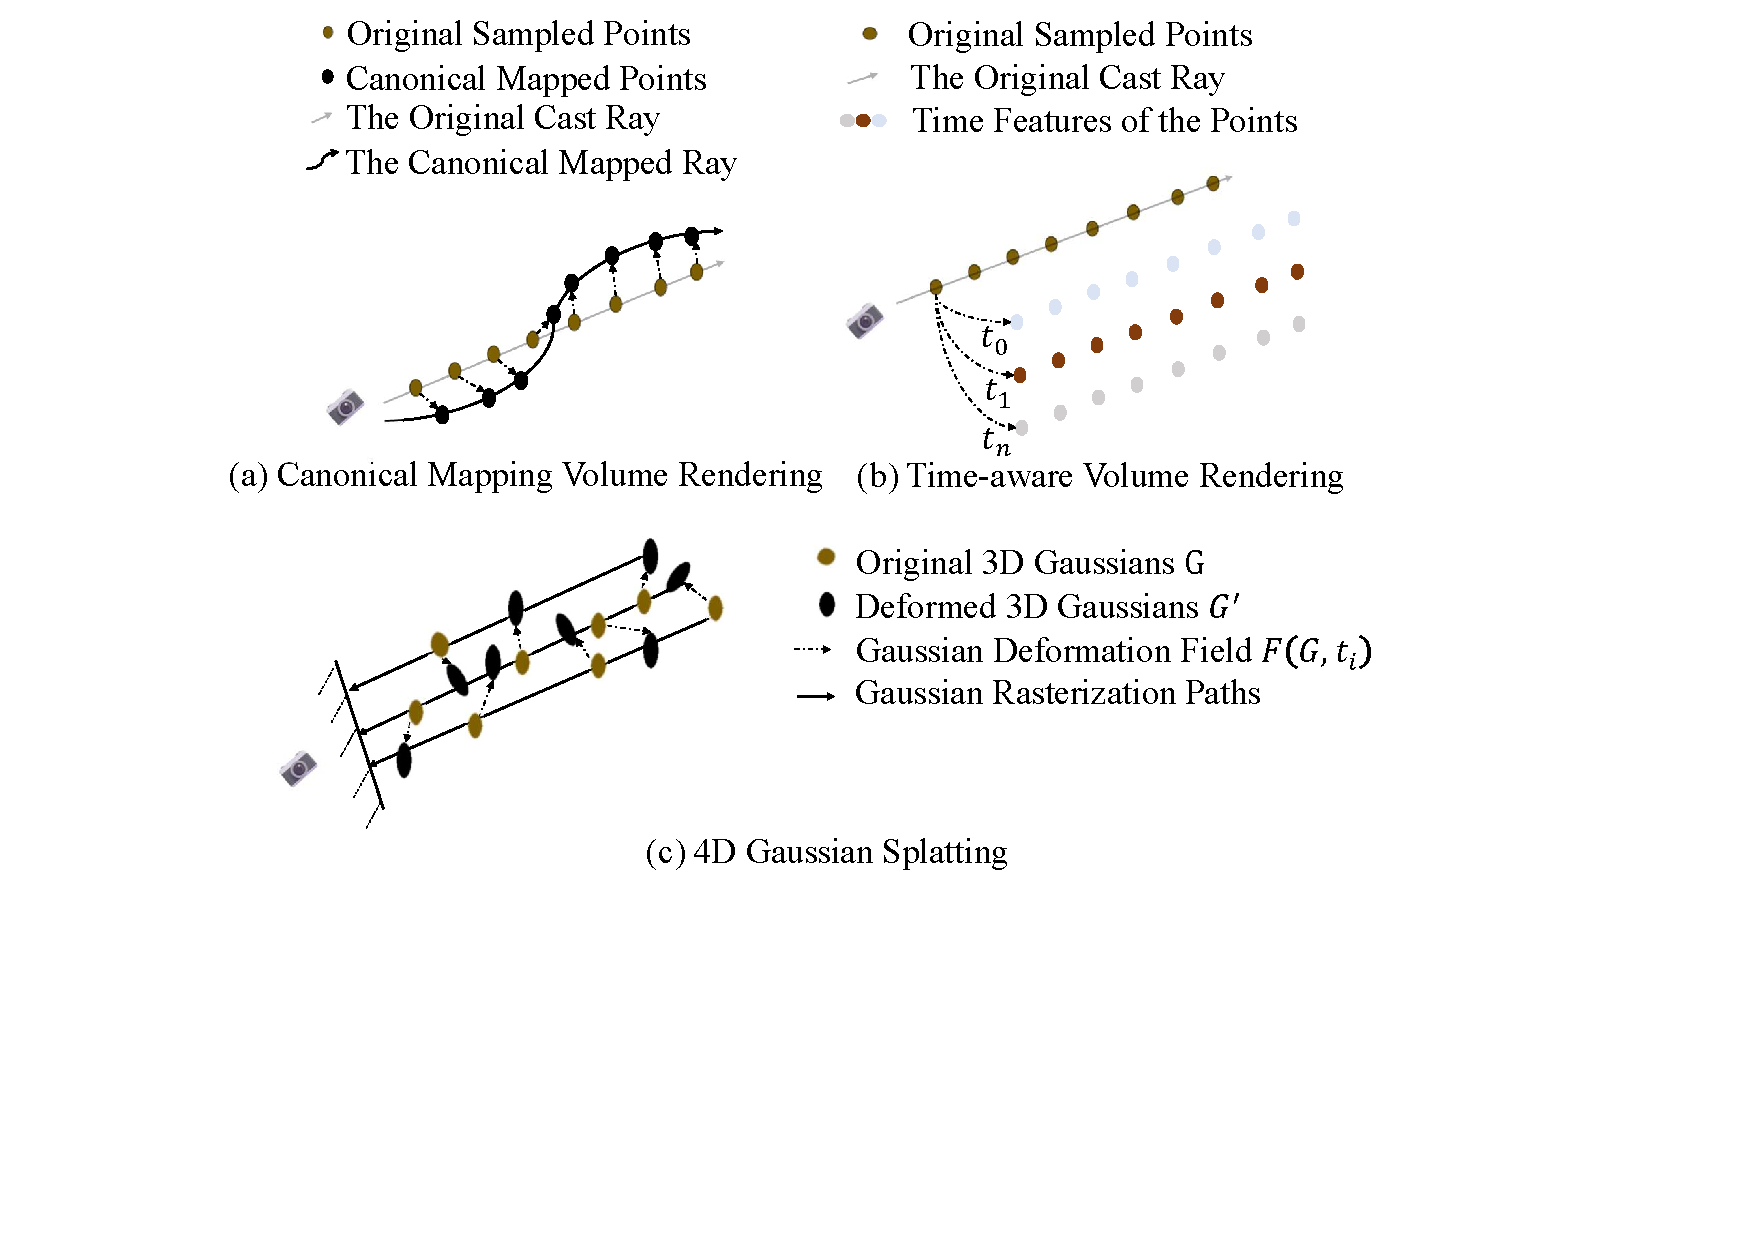
\includegraphics[width=1.0\linewidth]{fig/splatting_volume.pdf}
   \caption{Illustration of different dynamic scene rendering methods. (a) Points are sampled in the casted ray during volume rendering. The point deformation fields proposed in~\cite{pumarola2021dnerf, tineuvox} map the points into a canonical space. (b) Time-aware volume rendering computes the features of each point directly and does not change the rendering path. (c) The Gaussian deformation field converts original 3D Gaussians into another group of 3D Gaussians with a certain timestamp.}
   \label{fig: splatting-volume}
   \vspace{-10pt}
\end{figure}

\begin{figure*}[thbp]
   \centering
   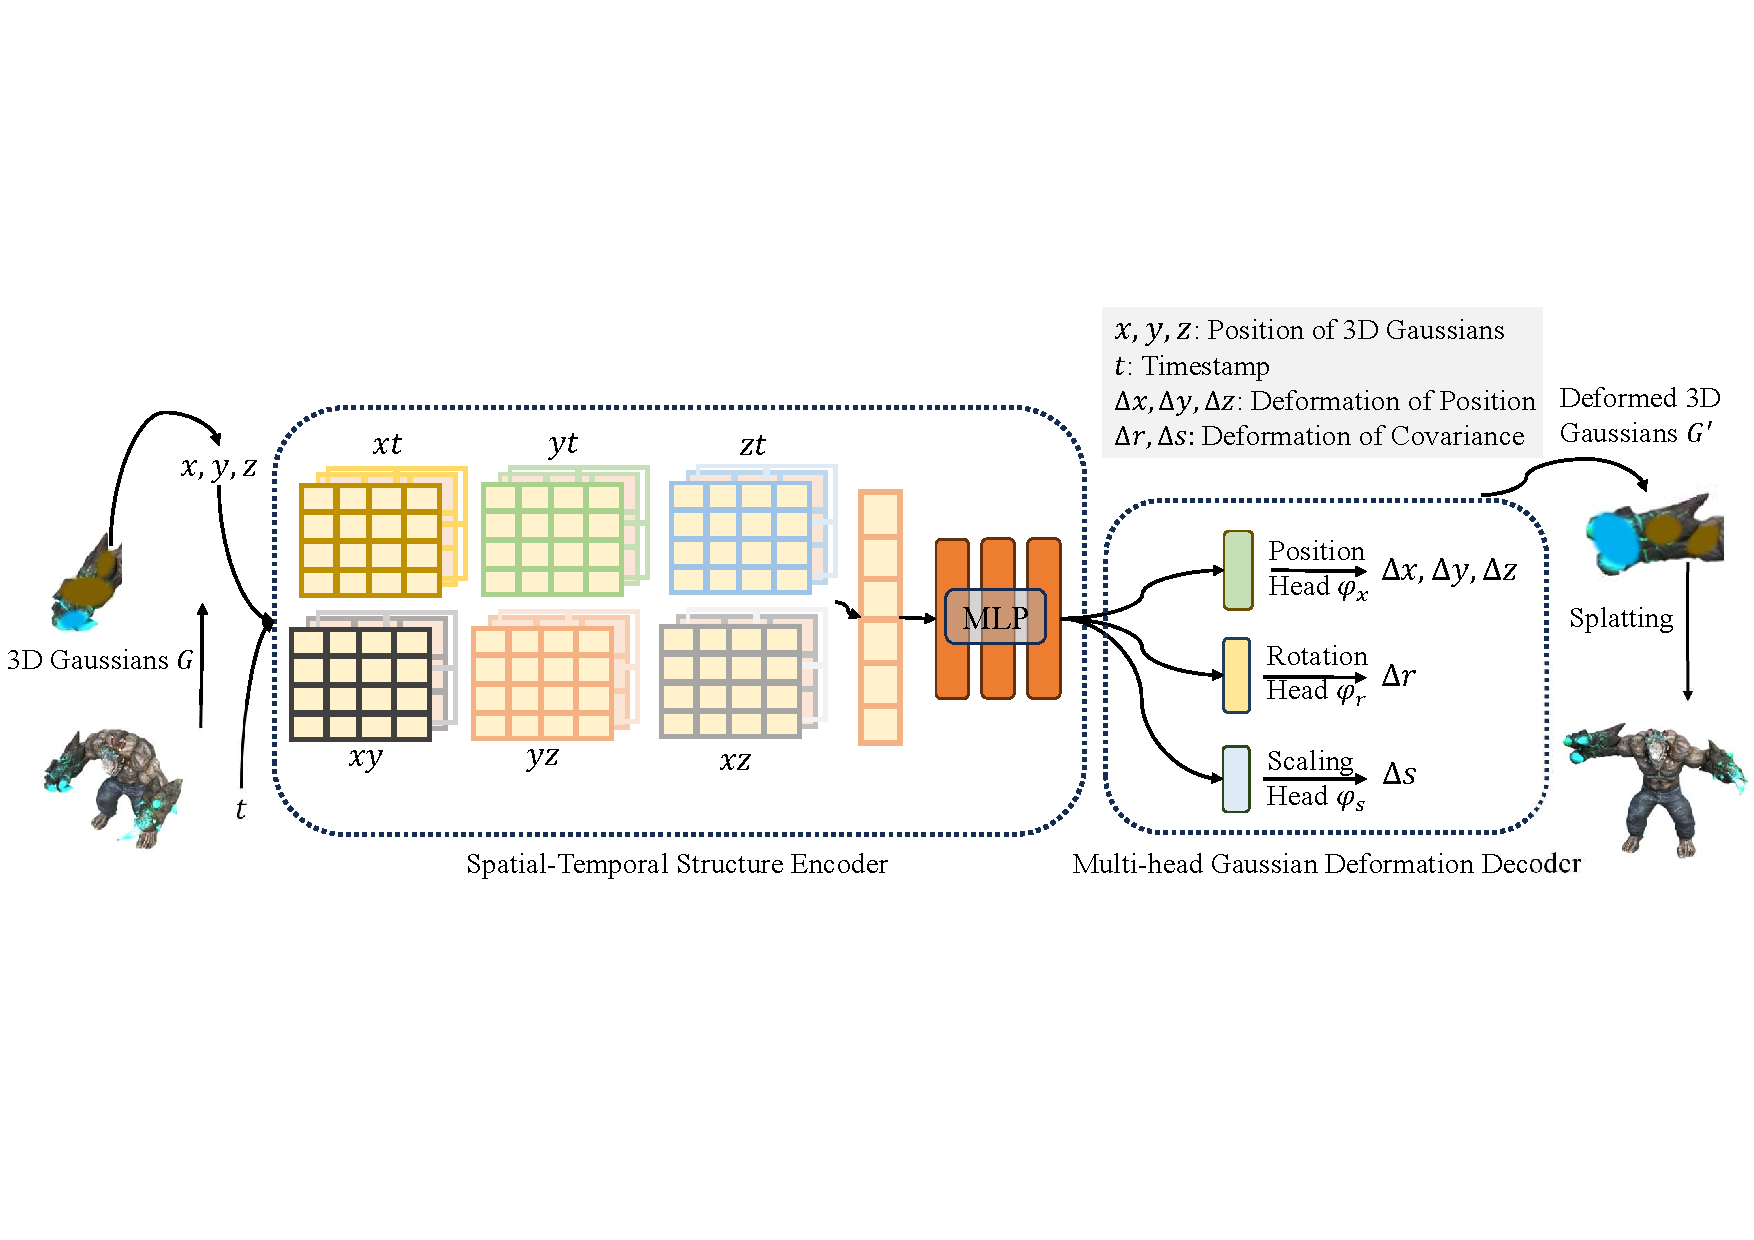
\includegraphics[width=1.0\linewidth]{fig/pipeline.pdf}
   \caption{The overall pipeline of our model. Given a group of 3D Gaussians $\mathcal{G}$, we extract the center coordinate of each 3D Gaussian $\mathcal{X}$ and timestamp $t$ to compute the voxel feature by querying multi-resolution voxel planes. Then a tiny multi-head Gaussian deformation decoder is used to decode the feature and get the deformed 3D Gaussians $\mathcal{G}^\prime$ at timestamp $t$. The deformed Gaussians are then splatted to the rendered image.}
   \label{fig: pipeline}
   \vspace{-10pt}
\end{figure*}
\section{Related Works}
In this section, we simply review the difference of dynamic NeRFs in Sec.~\ref{subsec:dynamic novel view synthesis}, then discuss the point clouds-based neural rendering algorithm in Sec.~\ref{subsec:neural rendering with point clouds}.

\subsection{Neural Rendering}
\label{subsec:dynamic novel view synthesis}
Light fields can efficiently render novel views with dense image input. Mesh-based representations succeed in maintaining real-time rendering with modern rasterization pipelines. Voxel grids and multi-plane images also support gradient optimization. \cite{mildenhall2021nerf,barron2021mip,zhang2020nerf++} demonstrate that implicit radiance fields can effectively learn scene representations and synthesize high-quality novel views.~\cite{pumarola2021dnerf,park2021nerfies,park2021hypernerf} have challenged the static hypothesis, expanding the boundary of novel view synthesis for dynamic scenes. Additionally,~\cite{tineuvox} proposes to use an explicit voxel grid to model temporal information, accelerating the learning time for dynamic scenes to half an hour and applied in~\cite{gneuvox,robustdynamicradiancefields,guo2023forwardflowfornvs}. The proposed canonical mapping neural rendering methods are shown in Fig.~\ref{fig: splatting-volume} \textcolor{red} {(a)}. ~\cite{li2022neural,hexplane,kplanes,tensor4d,msth} represent further advancements in faster dynamic scene learning by adopting decomposed neural voxels. They treat sampled points in each timestamp individually as shown in Fig.~\ref{fig: splatting-volume} \textcolor{red} {(b)}.~\cite{wang2023neus2,gao2022mps,mlpmaps,xu2022multigeometric,lin2023im4d,wang2023mixedvoxels} are efficient methods to handle multi-view setups. The aforementioned methods though achieve fast training speed, real-time rendering for dynamic scenes is still challenging, especially for monocular input. Our method aims at constructing a highly efficient training and rendering pipeline in Fig.~\ref{fig: splatting-volume} \textcolor{red} {(c)}, while maintaining the quality, even for sparse inputs.
% While the methods mentioned above offer fast training speeds, the process of rendering an image still cannot achieve real-time performance. Meanwhile, Our proposed method is an efficient solution to achieve both high-quality novel view synthesis and extremely fast rendering speed.

% \paragraph{Accelerating Neural Rendering.}\label{subsec:Accelerating Dynamic NeRF's Rendering Speed}
% \cite{yu2021plenoctrees,hedman2021baking,reiser2021kilonerf,fridovich2022plenoxels,dvgo,instantngp} use explicit representations or the baking method to promote the training and rendering speed but mainly focus on the static scenes. Some works~\cite{mlpmaps, wang2022fourierplenoctrees,lin2023im4d} aim at accelerating the rendering on dynamic scenes but multi-view setups are needed. It becomes a growing demand to achieve general real-time rendering methods for dynamic scenes at sparse sequential camera setups. 3D Gaussian Splatting (3D-GS)~\cite{3dgs}, an effective scene representation and rendering method, has been developed that not only achieves fast convergence speeds but is also easily integrated into the graphics rendering pipeline, making real-time rendering of general scenes more accessible. Our method extends 3D-GS~\cite{3dgs} to 4D, named 4D-GS, achieving real-time rendering for general dynamic scenes that can be applied easily with both monocular and multi-view input.

\subsection{Neural Rendering with Point Clouds}\label{subsec:neural rendering with point clouds}
Effectively representing 3D scenes remains a challenging topic. The community has explored various neural representations~\cite{mildenhall2021nerf}, \eg meshes, point clouds~\cite{pointnerf}, and hybrid approaches. Point-cloud-based methods~\cite{qi2017pointnet,qi2017pointnet++,yu2018pu,liu2019meteornet} initially target at 3D segmentation and classification. A representative approach for rendering presented in~\cite{pointnerf, abou2022particlenerf} combines point cloud representations with volume rendering, achieving rapid convergence speed.~\cite{keselman2023flexibleTechniquesDifferentiableRendering,keselman2022approximatedifferentiablerenderingwithalgebraicsurfaces,ruckert2022adop} adopt differential point rendering technique for scene reconstructions. Additionally, 3D-GS~\cite{3dgs} is notable for its pure explicit representation and differential point-based splatting methods, enabling real-time rendering of novel views. Dynamic3DGS~\cite{dynamic3dgs} models dynamic scenes by tracking the position and variance of each 3D Gaussian at each timestamp $t_i$. An explicit table is utilized to store information about each 3D Gaussian at every timestamp, leading to a linear memory consumption increase, denoted as $O(t\mathcal{N})$, in which $\mathcal{N}$ is num of 3D Gaussians. For long-term scene reconstruction, the storage cost will become non-negligible. The memory complexity of our approach only depends on the number of 3D Gaussians and parameters of Gaussians deformation fields network $\mathcal{F}$, which is denoted as $O(\mathcal{N}+\mathcal{F})$.~\cite{4dgs-2} adds a marginal temporal Gaussian distribution into the origin 3D Gaussians, which uplift 3D Gaussians into 4D. However, it may cause each 3D Gaussian to only focus on their local temporal space. Our approach also models 3D Gaussian motions but with a compact  network, resulting in highly efficient training efficiency and real-time rendering.  
